\documentclass[10pt]{SPIIRAS_Proceedings}

\graphicspath{{media/}}

\usepackage[%
  parentracker=true,
  style=gost-numeric,
  defernumbers=true,
  movenames=false,
  maxnames=100,
  % isbn=false,
  % doi=false,
  sorting=none,
]{biblatex}

% \toggletrue{bbx:gostbibliography}

\addbibresource{dombai.bib}

\udk{519.8.А}

\titleRus{
  Маршрутные процессы в задачах последовательного обхода множеств при наличии ограничений%
}

\authorsRus{
  А.А. Петунин,
  А.Г. Ченцов,
  П.А. Ченцов.
}

\authorsTitleRus{
  А.А. П\smallcapsfake{етунин},
  А.Г. Ч\smallcapsfake{енцов},
  П.А. Ч\smallcapsfake{енцов}
} % \smallcapfake необходим для имитации малых прописных букв ввиду отсутствия поддержки в используемом шрифте

\abstractRus{
  Исследуется задача маршрутизации перемещений с ограничениями и функциями стоимости,
  зависящими от списка заданий.
  Рассматриваемая постановка ориентирована на инженерные приложения,
  связанные с листовой резкой деталей на машинах с ЧПУ;
  возможны и другие применения
  (в частности, полученные результаты могут использоваться в задаче минимизации дозовой нагрузки
  при демонтаже системы радиационно опасных элементов при авариях на АЭС).
  Объектами посещения являются непустые конечные множества –- мегаполисы.
  Среди ограничений особо выделяются условия предшествования,
  которые удается использовать для снижения вычислительной сложности.
  В качестве основного метода исследования используется
  широко понимаемое динамическое программирование (ДП),
  учитывающее условия предшествования
  и зависимость функций стоимости от списка заданий.
  В процессе решения оптимизируются
  вариант очередности выполнения заданий,
  конкретная траектория процесса и точка старта.
  Алгоритм реализован в виде программы для ПЭВМ;
  решен модельный пример.
}

\keywordsRus{
    динамическое программирование,
    допустимое решение,
    маршрут,
    траектория
}

\begin{document}

\maketitle

\normalsize

\section*{Введение}
\label{sec:intro}

Объектом исследования в статье
являются задачи маршрутизации перемещений
с ограничениями различных типов;
среди последних особо выделяем условия
предшествования и ограничения динамического характера,
возникающие по мере развития процесса и проведения тех или иных работ.
При должной формализации возникает постановка,
идейно близкая к дискретным задачам управления большой размерности
(имеется в виду дискретность и по времени и  по фазовому состоянию).
Оптимизируется комплекс, включающий точку старта,
вариант очередности исполнения заданий
(далее -- маршрут)
и конкретную траекторию;
сам возникающий при этом комплекс (триплет)
именуем маршрутным процессом.
Возможные применения могут быть,
в частности, связаны с атомной энергетикой
(см. \cite{1,2,3};
задача минимизации дозовой нагрузки работников при демонтаже радиационно опасных объектов)
и машиностроением (см. \cite{4,5,6};
задача управления инструментом при фигурной листовой резке на машинах с ЧПУ);
имеются и другие приложения.
В настоящей статье ориентируемся на применение разрабатываемых методов в машиностроении;
следуем при этом монографии \cite{4}.
Здесь первоначальная задача управления режущим инструментом
с условиями предшествования и динамическими ограничениями
преобразуется к строгой математической постановке
оптимизационной задачи в классе вышеупомянутых маршрутных процессов,
в которой нашей целью является нахождение
глобального экстремума и соответствующего оптимального решения.
Кратко излагаются элементы общей теории и
конструируемый на ее основе оптимальный алгоритм,
реализованный на многоядерной ПЭВМ.
Используются понятия и обозначения
\cite[часть II]{4},
относящиеся к математической постановке,
а также содержательные построения \cite[часть I]{4}.

Рассматриваемая задача имеет своим прототипом известную труднорешаемую задачу коммивояжера
или TSP в англоязычной литературе; см. \cite{7,8,9,10,11,12}. Однако существенные особенности качественного характера (прежде всего, наличие ограничений) мотивируют построение специализированной теории; см. \cite{1,3,4,5,6,13,14}.
Разработке упомянутых теоретических вопросов посвящены, в частности, монографии \cite{13,14,14`}. В настоящем изложении мы выделяем \cite{4}, где на примере актуальной инженерной задачи удается продемонстрировать ряд принципиальных положений теоретического характера и, в частности, представить возможности динамического программирования (ДП) как общего метода решения различных прикладных задач.


\section{Сводка общих понятий}
\label{sec:1}

Используем стандартную теоретико множественную символику
(кванторы, связки и др.);
через $\varnothing$ обозначаем пустое множество,
$\stackrel{\triangle}{=}$ -- равенство по определению.
Множество, все элементы которого сами являются множествами,
называем семейством.
Если $x$ и $y$ -- объекты,
то $\{x;y\}$
есть их неупорядоченная пара:
$\{x;y\}$ содержит $x,\;y$
и не содержит никаких других элементов.
Для всякого объекта $z$ в виде $\{z\} \stackrel{\triangle}{=} \{z;z\}$
имеем синглетон,
содержащий $z$.
Множества являются объектами.
Если $a$ и $b$ -- объекты, то
\cite[c.~67]{15}
$(a,b) \stackrel{\triangle}{=} \{\{a\};\{a;b\}\}$
есть упорядоченная пара с первым элементом $a$ и вторым элементом $b$.
Для каждой упорядоченной пары $h$ через
$\mathrm{pr}_1(h)$ и $\mathrm{pr}_2(h)$
обозначаем первый и второй элементы $h$,
однозначно определяемые условием
$h = (\mathrm{pr} _1(h),\mathrm{pr} _1(h))$.
Если же $x,\;y$ и $z$ -- объекты,
то $(x,y,z) \stackrel{\triangle}{=} ((x,y),z)$
есть их упорядоченный триплет.
Соответственно,
$A \times B \times C = (A \times B) \times C$
для любых трех множеств $A,\;B$ и $C;$ см.
\cite[c.17]{16}.

Множеству $H$
сопоставляется семейство $\mathcal{P}(H)$
всех подмножеств (п/м) $H$
и $\mathcal{P}'(H) \stackrel{\triangle}{=}
\mathcal{P}(H) \setminus \{\varnothing\}$ -- семейство всех непустых п/м $H;$
через $\mathrm{Fin}(H)$
обозначаем семейство всех непустых конечных п/м
$H,\;\mathrm{Fin}(H) \subset \mathcal{P}'(H).$
Для непустого конечного множества $H$ имеем равенство
$\mathrm{Fin}(H) = \mathcal{P}'(H).$
Если $A$ и $B$ -- непустые множества,
$f$ -- отображение (функция) из $A$ в $B,$
а $C \in \mathcal{P}(A),$ то
$f^1(C) \stackrel{\triangle}{=} \{f(x):\;x \in C\} \in \mathcal{P}(B)$
есть образ $C$ при действии $f.$

Как обычно,
$\mathbb{R}$ -- вещественная прямая,
$\mathbb{R}_+ \stackrel{\triangle}{=} \{\xi \in \mathbb{R} \vert 0 \le \xi\} = [0,\infty[,\;\mathbb{N} \stackrel{\triangle}{=} \{1;2;...\}$
и $\mathbb{N}_0 \stackrel{\triangle}{=} \{0\} \cup \mathbb{N} = \{0;1;2;...\};$
при $p \in \mathbb{N}_0$ и $q \in \mathbb{N}_0$
$$
\overline{p,q} = \{\;k \in \mathbb{N}_0 \vert (p \le k) \& (k \le q)\}
$$
(при $q < p$ имеем $\overline{p,q} = \varnothing$).
Если $S$ -- непустое множество, то
$\mathcal{R}_+[S]$
есть множество всех неотрицательных вещественнозначных (в/з) функций на $S.$
Каждому непустому конечному множеству $K$
сопоставляем его мощность $|K| \in \mathbb{N}$
и непустое множество $(\mathrm{bi})[K]$
всех биекций
\cite[c.~87]{17} <<промежутка>>
$\overline{1,|K|}$ на $K;$
пусть
$|\varnothing| \stackrel{\triangle}{=} 0.$
Ясно, что при
$m \in \mathbb{N}$ в виде $(\mathrm{bi})[\overline{1,m}]$
имеем множество всех перестановок
\cite[c.~87]{17} множества
$\overline{1,m};$
если $\alpha \in (\mathrm{bi})[\overline{1,m}],$
то определена перестановка
$\alpha^{-1} \in (\mathrm{bi})[\overline{1,m}],$
обратная к
$\alpha:\;\alpha(\alpha^{-1}(k)) = \alpha^{-1}(\alpha(k)) = k$
при $k \in \overline{1,m}.$
Напомним, что здесь и ниже символика соответствует
\cite[$\S$3.1]{4}.

\section{Математическая постановка задачи}
\label{sec:2}

Фиксируем непустое множество $X$
(в содержательных задачах \cite{4}
$X$ -- прямоугольник на плоскости)
и $X^0 \in \mathrm{Fin}(X);$
в пределах $X$ осуществляются рассматриваемые перемещения,
для которых точки из $X^0$ играют роль стартовых.
Пусть $N \in \mathbb{N}$ таково,
что $2 \le N;$
фиксируем $N$ множеств
\begin{equation}\label{2.1}
M_1 \in \mathrm{Fin}(X),...,M_N \in \mathrm{Fin}(X),
\end{equation}
именуемых далее мегаполисами, а
также $N$ отношений (см. \cite[гл.II,$\S$4]{15})
\begin{equation}\label{2.2}
\mathbb{M}_1 \in \mathcal{P}'(M_1 \times M_1),...,\mathbb{M}_N \in \mathcal{P}'(M_N \times M_N).
\end{equation}

Мегаполисы (\ref{2.1})
являются объектами посещения,
а точки каждого отношения в (\ref{2.2})
определяют допустимые варианты выполнения работ,
связанных с посещением соответствующего мегаполиса и именуемых далее внутренними.
Полагаем, что
$M_j \cap X^0 = \varnothing$
при
$j \in \overline{1,N};$
кроме того, пусть $M_p \cap M_q = \varnothing$
при $p \in \overline{1,N},\;q \in \overline{1,N},\;p \ne q.$
Если $j \in \overline{1,N},$
то полагаем, что
\begin{equation}\label{2.3}
(\mathfrak{M}_j \stackrel{\triangle}{=}
\{\;\mathrm{pr}_1(z):\;z \in \mathbb{M}_j\})
\& (\mathbf{M}_j \stackrel{\triangle}{=}
\{\;\mathrm{pr}_2(z):\;z \in \mathbb{M}_j\});
\end{equation}

В (\ref{2.3}) указаны множества возможных пунктов прибытия в $M_j$
и отправления из $M_j$ соответственно.
В связи с (\ref{2.3})
отметим, что
$$
(\mathbb{X} \stackrel{\triangle}{=} X^0 \cup
(\bigcup\limits_{i=1}^n \mathfrak{M}_i) \in \mathrm{Fin}(X))
\& (\mathbf{X} = X^0 \cup (\bigcup\limits_{i=1}^N \mathbf{M}_i) \in \mathrm{Fin}(X)).
$$
Рассматриваемые ниже системы перемещений имеют вид
\begin{equation}\label{2.4}
  \begin{aligned}
    (x \in X^0)
    \to
    (x_{1,1} \in \mathfrak{M}_{\alpha(1)} \leadsto x_{1,2} \in \mathbf{M}_{\alpha(1)})
    \to \dots \\
    \to
    (x_{N,1} \in \mathfrak{M}_{\alpha(N)} \leadsto x_{N,2} \in \mathbf{M}_{\alpha(N)}),
  \end{aligned}
\end{equation}
где $\alpha$ -- перестановка $\overline{1,N},$
сплошные стрелки обозначают внешние перемещения,
а волнистые -- перемещения при выполнении внутренних работ;
в (\ref{2.4}) постулируется, что
\begin{equation}\label{2.5}
  (x_{1,1},x_{1,2}) \in \mathbb{M}_{\alpha(1)},
  \dots,
  (x_{N,1},x_{N,2}) \in \mathbb{M}_{\alpha(N)}.
\end{equation}

Мы рассматриваем (\ref{2.4}), (\ref{2.5})
как реализацию маршрутного процесса.
Выбор самого этого процесса должен удовлетворять
ряду условий,
среди которых особо выделяются условия предшествования (см.\cite{10}).
Для введения этих условий полагаем сначала,
что $\mathbb{P} \stackrel{\triangle}{=} (
  \mathrm{bi})[\overline{1,N}],$
так что в (\ref{2.4}), (\ref{2.5})
$\alpha \in \mathbb{P}.$
Фиксируем множество
$\mathbf{K} \in \mathcal{P}(\overline{1,N} \times \overline{1,N}),$
элементы которого
(а это упорядоченные пары)
называем адресными парами
(итак, $\mathbf{K} \subset \overline{1,N} \times \overline{1,N}$);
полагаем, что
\begin{equation}\label{2.6}
\forall{\mathbf{K}_0} \in \mathcal{P}'(\mathbf{K})\;\exists{z_0} \in \mathbf{K}_0:\;\mathrm{pr}_1(z_0)
\ne \mathrm{pr}_2(z)\;\;\forall{z} \in \mathbf{K}_0.
\end{equation}

Первый элемент адресной пары часто называют отправителем,
а второй -- получателем
(груза, сообщения и др.).
Тогда, как показано в \cite[часть 2]{14},
\begin{multline}\label{2.7}
  % \begin{aligned}
    \mathbf{A} \stackrel{\triangle}{=} \\
    \left\{\;\alpha \in \mathbb{P} \vert\;
      \forall{t_1} \in \overline{1,N}\;\
      \forall{t_2}  \in \overline{1,N}\;\;
      ((\alpha(t_1),\alpha(t_2)) \in \mathbf{K})
      \Longrightarrow (t_1 < t_2)
    \right\} = \\
    =
    \left\{\;
      \alpha \in \mathbb{P} \vert
      \alpha^{-1}(\mathrm{pr}_1(z)) < \alpha^{-1}(\mathrm{pr}_2(z))\;\;\forall{z}
      \in \mathbf{K}
    \right\} \ne \varnothing
  % \end{aligned}
\end{multline}
есть (при условии (\ref{2.6}))
непустое множество всех маршрутов
(следуем терминологии TSP,
называя маршрутами перестановки индексов из $\overline{1,N}$),
допустимых по предшествованию или $\mathbf{K}$-допустимых:
имеются в виду маршруты,
для которых у любой адресной пары мегаполис-отправитель посещается раньше,
чем мегаполис-получатель.
Возвращаясь к (\ref{2.4}),
введем в рассмотрение траектории,
согласованные с маршрутами.
Сначала введем в рассмотрение множество
$\mathbb{Z}$ всех кортежей
$(z_i)_{i \in \overline{0,N}}: \overline{0,N} \longrightarrow \mathbb{X} \times \mathbf{X}.$
Если $x \in X^0$ и $\alpha \in \mathbb{P},$
то
\begin{equation}\label{2.8}
\mathcal{Z}_\alpha[x] \stackrel{\triangle}{=} \{(z_i)_{i \in \overline{0,N}}
\in \mathbb{Z} \vert\;(z_0 = (x,x)) \& (z_t \in \mathbb{M}_{\alpha(t)}\;\forall{t} \in \overline{1,N})\} \in \mathrm{Fin}(\mathbb{Z}).
\end{equation}

Из (\ref{2.8}) видно,
что траектории из
$\mathcal{Z}_\alpha[x]$
реализуют в строгой форме схему (\ref{2.4}), (\ref{2.5}).
При $x \in X^0$
получаем, что
\begin{equation}\label{2.9}
  \tilde{D}[x] \stackrel{\triangle}{=}
  \{(\alpha,(z_i)_{i \in \overline{0,N}}) \in \mathbf{A} \times \mathbb{Z}
  \vert \;(z_i)_{i \in \overline{0,N}} \in \mathcal{Z}_\alpha[x]\}
  \in \mathrm{Fin}(\mathbf{A} \times \mathbb{Z});
\end{equation}
(\ref{2.9}) есть множество всех допустимых решений (ДР)
частной задачи со стартом из $x,$ или $x$-задачи.
Наконец,
\begin{multline}\label{2.10}
  \mathbf{D} \stackrel{\triangle}{=}
  \{(\alpha,(z_i)_{i \in \overline{0,N}},x) \in \mathbf{A} \times \mathbb{Z} \times X^0 \vert
  (\alpha,(z_i)_{i \in \overline{0,N}}) \in \tilde{D}[x]\}
  \in
  \\
  \in \mathrm{Fin}(\mathbf{A} \times \mathbb{Z} \times X^0),
\end{multline}
получая множество всех ДР формулируемой ниже полной задачи.

{\bf Функции стоимости.}
Через $\mathfrak{N}$
обозначим семейство всех непустых п/м
$\overline{1,N}:\;\mathfrak{N} \stackrel{\triangle}{=}  \mathcal{P}'(\overline{1,N}).$
Фиксируем $N + 2$ функции
\begin{equation}\label{2.11}
  \mathbf{c} \in \mathcal{R}_+[\mathbf{X} \times \mathbb{X} \times \mathfrak{N}],\;
  c_1 \in \mathcal{R}_+[\mathbb{M}_1 \times \mathfrak{N}],...,
  c_N \in \mathcal{R}_+[\mathbb{M}_N \times \mathfrak{N}],\;
  f \in \mathcal{R}_+[\mathbf{M}],
\end{equation}
где $\mathbf{M}$
есть объединение всех множеств
$\mathbf{M}_i,\;i \in \overline{1,N}.$

Полагаем, что функция $\mathbf{c}$ оценивает внешние перемещения,
т.е. перемещения между мегаполисами,
а также из точек множества $X^0$ к мегаполисам.
При $j \in \overline{1,N}$
функция $c_j$
оценивает выполнение внутренних работ,
связанных с посещением $M_j.$
Наконец, функция $f$
оценивает терминальное состояние
(точка $x_{N,2}$
в (\ref{2.5})).
Как видно из (\ref{2.11})
одним из аргументов функций $\mathbf{c},c_1,...,c_N$
является элемент семейства $\mathfrak{N},$
т.е. непустое п/м $\overline{1,N},$
именуемое далее списком (заданий).
В последующих теоретических построениях
в этом качестве будет использоваться список заданий,
не выполненных на текущий момент времени,
что характерно для задач о демонтаже,
связанных с обслуживанием АЭС и ликвидаций возможных аварий;
см. \cite{1,2,3}.
В случае фигурной листовой резки
(см. \cite{4}) возникает
(в связи с динамическими ограничениями)
необходимость использования зависимости
от списка уже выполненных заданий;
таким образом, вводя надлежащие штрафы,
удается учитывать ограничения динамического характера
(см. \cite{18}).
Однако, вводя дополнение такого списка до
$\overline{1,N},$
можно и этот случай свести к применению зависимостей
(\ref{2.11}).

В дальнейшем оптимизируется аддитивный критерий,
для введения которого полагаем,
что при
$x \in X^0,\;\alpha \in \mathbb{P}$ и
$(z_i)_{i \in \overline{1,N}} \in \mathcal{Z}_\alpha[x]$
\begin{multline}\label{2.12}
\mathfrak{C}_{\alpha}[(z_i)_{i \in \overline{1,N}}] \stackrel{\triangle}{=}
\\
\sum\limits_{i=1}^N [\mathbf{c}(\mathrm{pr}_2(z_{i-1}),\mathrm{pr}_1(z_i),\alpha^1(\overline{i,N})) +
c_{\alpha(i)}(z_i,\alpha^1(\overline{i,N}))] +
\\
+ f(\mathrm{pr}_2(z_N));
\end{multline}

Итак, в (\ref{2.12})
мы суммируем затратные показатели для внешних перемещений,
для внутренних работ и терминального состояния
(в случае листовой резки один из важных вариантов (\ref{2.12})
есть совокупное время выполнения всех заданий;
здесь, однако,
возникает существенное преобразование постановки
в сравнении с исходной содержательной задачей
уже на этапе сведения к схеме
(\ref{2.4}), (\ref{2.5}); см. \cite[$\S$3.3]{4}).
C учетом (\ref{2.12}) получаем при
$x \in X^0$ частную задачу ($x$-задачу)
\begin{equation}\label{2.13}
  \mathfrak{C}_{\alpha}[(z_i)_{i \in \overline{0,N}}] \longrightarrow
  \mathrm{min},\;\;(\alpha,(z_i)_{i \in \overline{0,N}}) \in \tilde{D}[x],
\end{equation}
которая характеризуется экстремумом $V[x]$
(наименьшее из чисел
$\mathfrak{C}_{\alpha}[(z_i)_{i \in \overline{0,N}}],\;(\alpha,(z_i)_{i \in \overline{0,N}}) \in \tilde{D}[x])$
и множеством
\begin{equation}\label{2.14}
  (\mathrm{SOL})[x] \stackrel{\triangle}{=}
  \{\;(\alpha^0,(z_i^0)_{i \in \overline{0,N}}) \in \tilde{D}[x] \vert
  \mathfrak{C}_{\alpha^0}[(z_i^0)_{i \in \overline{0,N}}] = V[x]\} \in \mathcal{P}'(\tilde{D}[x])
\end{equation}
всех оптимальных
(при старте из $x$)
решений; (\ref{2.14}) -- непустое конечное множество.
В виде
\begin{equation}\label{2.15}
  \mathfrak{C}_{\alpha}[(z_i)_{i \in \overline{0,N}}] \longrightarrow
  \mathrm{min},\;\;(\alpha,(z_i)_{i \in \overline{0,N}},x) \in \mathbf{D},
\end{equation}
имеем полную задачу, характеризуемую (глобальным) экстремумом
\begin{equation}\label{2.16}
  \mathbb{V} \stackrel{\triangle}{=}
  \min\limits_{(\alpha,(z_i)_{i \in \overline{0,N}},x) \in
  \mathbf{D}}\mathfrak{C}_{\alpha}[(z_i)_{i \in \overline{0,N}}]
  = \min\limits_{x \in X^0} V[x] \in \mathbb{R}_+
\end{equation}
и (непустым конечным) экстремальным множеством
\begin{equation}\label{2.17}
  \mathbf{SOL} \stackrel{\triangle}{=}
  \{\;(\alpha,(z_i)_{i \in \overline{0,N}},x) \in \mathbf{D}
  \vert \mathfrak{C}_{\alpha}[(z_i)_{i \in \overline{0,N}}] =
  \mathbb{V}\} \in \mathrm{Fin}(\mathbf{D}).
\end{equation}

В связи с (\ref{2.16})
отметим также следующую задачу оптимизации точки старта
\begin{equation}\label{2.18}
  V[x] \longrightarrow \mathrm{min},\;\;x \in X^0,
\end{equation}
имеющую экстремум $\mathbb{V}$
(см. (\ref{2.16})) и экстремальное множество
\begin{equation}\label{2.19}
  X^0_{\mathrm{opt}} \stackrel{\triangle}{=} \{\;x^0 \in X^0 \vert V[x^0] = \mathbb{V}\} \in \mathcal{P}'(X^0).
\end{equation}

\begin{proposition}
\label{prop:2.1}
Если
$x^0 \in X^0_{\mathrm{opt}}$ и $(\alpha^0,(z_i^0)_{i \in \overline{0,N}}) \in (\mathrm{SOL})[x^0],$
то
\begin{equation}\label{2.20}
  (\alpha^0,(z_i^0)_{i \in \overline{0,N}},x^0) \in \mathbf{SOL}.
\end{equation}
\end{proposition}

\begin{proof}

Фиксируем $x^0$ и $(\alpha^0,(z_i^0)_{i \in \overline{0,N}})$
в соответствии с условиями.
Тогда (см. (\ref{2.19}))
$V[x^0] = \mathbb{V},$
\begin{equation}\label{2.21}
 (\alpha^0,(z_i^0)_{i \in \overline{0,N}}) \in \tilde{D}[x^0].
\end{equation}

В частности,
$(\alpha^0,(z_i^0)_{i \in \overline{0,N}}) \in \mathbf{A} \times \mathbb{Z}$
обладает свойством
$(z_i^0)_{i \in \overline{0,N}} \in \mathcal{Z}_{\alpha^0}[x^0].$
Тогда
$(\alpha^0,(z_i^0)_{i \in \overline{0,N}},x^0) \in \mathbf{D}$
в силу (\ref{2.10}), (\ref{2.19}) и (\ref{2.21}).
При этом согласно (\ref{2.14})
имеем по выбору $x^0,$ что
$$
  \mathfrak{C}_{\alpha^0}[(z_i^0)_{i \in \overline{0,N}}] = V[x^0] = \mathbb{V}.
$$

С учетом (\ref{2.17}) получаем теперь нужное свойство (\ref{2.20}).
\hfill $\Box$
\end{proof}

Из предложения \ref{prop:2.1} вытекает,
что решение задачи (\ref{2.15})
можно искать по следующей схеме:
1) нахождение $x^0 \in X^0_{\mathrm{opt}};$
2) решение задачи (\ref{2.13}) при $x = x^0;$
3) использование (\ref{2.20}).

\section{Конкретизация общей постановки}
\label{sec:3}

Совсем кратко напомним некоторые построения \cite[$\S$ 3.3]{4}.
Полагаем здесь, что $X$ -- прямоугольник на плоскости:
$X = [0,a] \times [0,b]$,
где $a \in \mathbb{R}_+ \setminus \{0\}$ и $b \in \mathbb{R}_+ \setminus \{0\}.$
Итак, $a > 0$ и $b > 0.$
Имеется раскройный план;
намечены контура попарно дизъюнктных деталей.
У каждой детали имеется один внешний и,
возможно,
несколько внутренних контуров
(см. \cite[\S~3.2]{4}).
Реально контура окружены близкими к ним эквидистантами.
Однако сейчас для простоты
будем считать их совпадающими с контурами,
то есть будем говорить о резке по контурам.
По технологическим соображениям
резка внутренних контуров детали
(если они есть)
должна предшествовать резке внешнего контура.
Возникает естественный вариант условий предшествования.
В интересах компьютерной реализации считаем,
что возле каждого контура намечены возможные
точки врезки и соответствующие им точки выключения инструмента:
процедура врезки должным образом дискретизируется.
В результате возникают непустые конечные множества --
мегаполисы,
элементами которых являются точки врезки
и точки выключения инструмента.
Точки этих двух типов группируются в пары.
Для каждого мегаполиса
$M_j$
отношение
$\mathbb{M}_j$
состоит из упорядоченных пар;
элементами каждой такой пары является
точка врезки
и соответствующая ей точка выключения инструмента.

Выше уже отмечался один вариант
условий предшествования.
Возможны и другие варианты,
например,
может использоваться правило:
сначала режутся <<большие>> детали.
Из других ограничений сейчас отметим
тепловые допуски
(см. \cite{18}).
Имеется в виду обеспечение ситуации,
при которой возле точек врезки сохранялось бы
достаточное <<количество>>
невырезанного металла с тем,
чтобы обеспечивался удовлетворительный отвод тепла
(имеется в виду случай термической резки).
Более подробное описание см. в \cite{18}.

В рассматриваемой модели резки
по замкнутому контуру
на этапе математической постановки исключено
собственно время резки контуров,
поскольку оно одинаково для всех вариантов решения
и может быть легко учтено введением
дополнительного слагаемого.

Функция стоимости внешних перемещений
определена как время,
затрачиваемое в режиме холостого хода.
Аналогично оценивается терминальное состояние:
учитывается время перемещения до точки парковки
в режиме холостого хода.
Стоимость внутренних работ
получается суммированием двух компонент.
Одна из них определяется суммой времен,
затрачиваемых на перемещение
от точки врезки до точки начала реза,
и от последней до точки выключения инструмента
(перемещение в металле со скоростью рабочего хода).
Вторая компонента определяется функцией штрафа и
<<включается>> при нарушении тепловых допусков.
Предполагается, что точка начала реза
сопоставляется каждой паре с элементами в виде
точки врезки и точки выключения инструмента.
Таким образом
формируется значение (\ref{2.12})
для каждого маршрутного процесса.
Более подробные сведения см. в
\cite[часть 1, глава 3]{4}
и в
\cite{18}.

\section{Динамическое программирование (алгоритмический вариант)}
\label{sec:4}

Вернемся к весьма общей постановке раздела \ref{sec:2}.
Она опирается на общие положения, установленные в \cite{19,20}
и восходящие к \cite[$\S$4.9]{14}.
Мы ограничимся сейчас изложением в форме алгоритма на функциональном уровне,
выделяя основные этапы построения.
Прежде всего введем оператор вычеркивания
(заданий из списка)
$\mathbf{I},$ действующий в $\mathfrak{N}$ по правилу:
для
$K \in \mathfrak{N}$ список $\mathbf{I}(K) \in \mathfrak{N}$
определяется следующим образом:
\begin{equation}\label{4.1}
  \mathbf{I}(K) \stackrel{\triangle}{=} K \setminus \{\;\mathrm{pr}_2(z):\;z \in \Sigma[K]\},
\end{equation}
где
$\Sigma[K] \stackrel{\triangle}{=} \{z \in \mathbf{K} \vert (\mathrm{pr}_1(z) \in K) \& (\mathrm{pr}_2(z) \in K)\}.$
Cвойства данного оператора подробно рассматриваются в \cite[часть 2]{14}
(см., в частности, \cite[раздел 2.2]{14}).

1) {\bf Построение существенных списков заданий.}
Полагаем, что
\begin{equation}\label{4.2}
  \mathcal{G} \stackrel{\triangle}{=} \{\;K \in \mathfrak{N} \vert
  \forall{z} \in \mathbf{K}\;\;(\mathrm{pr}_1(z) \in K) \Longrightarrow (\mathrm{pr}_2(z) \in K)\}.
\end{equation}

Множества -- элементы семейства (\ref{4.2}) --
называем существенными списками
(см. \cite[раздел 4.9]{14}).
Введем ранжирование по мощности:
$\mathcal{G}_s \stackrel{\triangle}{=} \{\;K \in \mathcal{G} \vert s = |K|\}\;\;\forall{s} \in \overline{1,N}.$
Тогда
$\{\mathcal{G}_1;...;\mathcal{G}_N\}$
есть разбиение
$\mathcal{G},\;\mathcal{G}_N = \{\overline{1,N}\}$
(синглетон)
и
$\mathcal{G}_1 = \{\;\{t\}:\;t \in \overline{1,N} \setminus \mathbf{K}_1\},$
где
\begin{equation}\label{4.3}
  \mathbf{K}_1 = \{\;\mathrm{pr}_1(z):\;z \in \mathbf{K}\}.
\end{equation}

Наконец,
$\mathcal{G}_{s-1} = \{\;K \setminus\{t\}:\;K \in \mathcal{G}_s,\;t \in \mathbf{I}(K)\}$ при $s \in \overline{2,N};$
см. \cite[$\S$3.5]{4}.
Итак, получили рекуррентную процедуру построения существенных списков
$$
  \mathcal{G}_N \longrightarrow \mathcal{G}_{N-1} \longrightarrow ... \longrightarrow \mathcal{G}_1.
$$

2) {\bf Построение слоев пространства позиций.}
Конструируем (см. \cite[$\S$4.9]{14})
множества $D_0,D_1,...,D_N,$
элементами которых являются пары
$(x,K),\;x \in \mathbf{X},\;K \in \mathcal{G},$
называемые позициями.
Полагаем (см. (\ref{4.3}))
\begin{equation}\label{4.3'}
  (D_N \stackrel{\triangle}{=} \{\;(x,\overline{1,N}):\;x \in X^0\}) \&
  (D_0 \stackrel{\triangle}{=} \{\;(x,\varnothing):\;x \in
    \bigcup\limits_{i \in \overline{1,N} \setminus \mathbf{K}_1} \mathbf{\mathbf{M}}_i\}.
\end{equation}

Если
$s \in \overline{1,N-1}$ и $K \in \mathcal{G}_s,$
то последовательно строим
\begin{multline*}
  \mathcal{J}_s(K) \stackrel{\triangle}{=}
  \{\;j \in \overline{1,N} \setminus K \vert \{j\} \cup K
  \in \mathcal{G}_{s+1}\},
  \\
  \mathcal{M}_s[K] \stackrel{\triangle}{=}
  \bigcup\limits_{j \in \mathcal{J}_s(K)} \mathbf{M}_j,
  \\
  \mathbb{D}_s[K] \stackrel{\triangle}{=}
  \{(x,K):\;x \in \mathcal{M}_s[K]\}.
\end{multline*}

Полагаем теперь, что при $s \in \overline{1,N - 1}$
$$
  D_s \stackrel{\triangle}{=} \bigcup\limits_{K \in \mathcal{G}_s} \mathbb{D}_s[K].
$$

Итак, все множества
$D_0,D_1,...,D_N$ определены.
Все они непусты
(см. \cite[предложение 4.9.3]{14}
при несложной коррекции обозначений,
а также \cite{21}).
Отметим легко проверяемое ключевое свойство
\begin{equation}\label{4.4}
  (\mathrm{pr}_2(z),K \setminus \{j\}) \in D_{s-1}\;\;
  \forall{s} \in \overline{1,N}\;\forall{(x,K)} \in D_s\;
  \forall{j} \in \mathbf{I}(K)\;\forall{z} \in \mathbb{M}_j.
\end{equation}

3) {\bf Построение слоев функции Беллмана.}
Последовательно строим функции
$v_0 \in \mathcal{R}_+[D_0],\;v_1 \in \mathcal{R}_+[D_1],...,v_N \in \mathcal{R}_+[D_N].$
В рамках нашего алгоритма построение упомянутых функций (слоев)
осуществляется посредством рекуррентной процедуры
(см. \cite[$\S$4.9]{14}, \cite{18,19,20,21}).
Определяем функцию $v_0$ условием
\begin{equation}\label{4.5}
  v_0(x,\varnothing) \stackrel{\triangle}{=} f(x)\;\;
  \forall{x} \in \bigcup\limits_{i \in \overline{1,N} \setminus \mathbf{K}_1} \mathbf{\mathbf{M}}_i;
\end{equation}
учитываем при этом второе соотношение в (\ref{4.3'}).
Пусть $s \in \overline{1,N}$
и функция
$v_{s-1} \in \mathcal{R}_+[D_{s-1}]$
уже построена.
С учетом (\ref{4.4}) имеем, что определены все значения
$$
  v_{s-1}(\mathrm{pr}_2(z),K \setminus \{j\}) \in \mathbb{R}_+,\;
  (x,K) \in D_s,\;j \in \mathbf{I}(K),\;z \in \mathbb{M}_j.
$$

С учетом этого определяем функцию
$v_s \in \mathcal{R}_+[D_s]$
посредством следующего правила
\begin{multline}
  \label{4.6}
  v_s(x,K) \stackrel{\triangle}{=} \\
  \min\limits_{j \in \mathbf{I}(K)} \min\limits_{z \in \mathbb{M}_j}
  [\mathbf{c}(x,\mathrm{pr}_1(z),K) + c_j(z,K) + v_{s-1}(\mathrm{pr}_2(z),K \setminus \{j\})] \\
  \forall{(x,K)} \in D_s;
\end{multline}
см., в частности,
\cite[(4.3.13)]{4}.
Итак, (\ref{4.6})
определяет преобразование $v_{s-1}$ в $v_s.$
Мы получаем рекуррентную процедуру
\begin{equation}\label{4.7}
  v_0 \longrightarrow v_1 \longrightarrow ... \longrightarrow v_N.
\end{equation}

{\bf Замечание 4.1.}
Важно отметить, что (как и в \cite{22} для несколько иной задачи)
реализация (\ref{4.7}) требует сохранения на каждом шаге в памяти компьютера только одной из функций
$v_0,v_1,...,v_N.$
В самом деле, при
$s \in \overline{1,N}$
для построения $v_s$ требуется только функция $v_{s-1},$
массив значений которой и должен находиться в памяти компьютера.
Это обстоятельство определяет более экономичный
(с точки зрения ресурсов памяти)
вариант процедуры (\ref{4.7}).
Заметим, однако, что для построения оптимального решения потребуются уже все вышеупомянутые функции.

Возвращаясь к общему варианту (\ref{4.7}),
отметим, что финалом данной процедуры является построение функции
$v_N \in \mathcal{R}_+[D_N].$
Важно отметить, что
\begin{equation}\label{4.8}
  V[x] = v_N(x,\overline{1,N})\;\;\forall{x} \in X^0.
\end{equation}

Данное свойство является следствием того,
что все функции в (\ref{4.7}) являются сужениями единой функции Беллмана
(функции оптимального результата)
на слои пространства позиций.
В этой связи отметим \cite[$\S$4.9]{14}, \cite{18}
(см. также \cite[(4.3.1)]{4}).
Из (\ref{4.6}), (\ref{4.8})
имеем при
$x \in X^0,$ что (см. (\ref{4.3'}))
\begin{multline}
  \label{4.9'}
  V[x] = \\
  \min\limits_{j \in \mathbf{I}(\overline{1,N})} \min\limits_{z \in \mathbb{M}_j}
  [\mathbf{c}(x,\mathrm{pr}_1(z),\overline{1,N}) + c_j(z,\overline{1,N}) + v_{N-1}(\mathrm{pr}_2(z),\overline{1,N} \setminus \{j\})].
\end{multline}

Особо отметим, что в случае, когда требуется найти не только глобальный экстремум и оптимальную точку старта,
но и построить само оптимальное решение, при реализации (\ref{4.7})
в памяти компьютера требуется сохранять массивы значений всех функций
$v_0,v_1,...,v_N$
(в этой связи см. (\ref{4.9'})).

4) {\bf Нахождение оптимальной точки старта.}
В силу (\ref{4.8}) после реализации процедуры (\ref{4.7}) мы располагаем зависимостью
$$
  x \longmapsto V[x]:\;X^0 \longrightarrow \mathbb{R}_+;
$$
данная зависимость полностью определяется функцией $v_N.$
Поэтому для решения задачи (\ref{2.18}) следует проминимизировать
$v_N.$
В самом деле, используя (\ref{2.16}) и (\ref{4.8}) определяем
$\mathbb{V}$ по правилу
\begin{equation}\label{4.9}
  \mathbb{V} = \min\limits_{x \in X^0} v_N(x,\overline{1,N}),
\end{equation}
а точку
$x^0 \in X^0_{\mathrm{opt}}$
находим из условия:
$x^0 \in X^0$ и при этом
\begin{equation}\label{4.10}
  \mathbb{V} = v_N(x^0,\overline{1,N}).
\end{equation}

Таким образом, на основе (\ref{4.7}) удается
(см. (\ref{4.9}),(\ref{4.10})) решить задачу (\ref{2.18}),
причем сделать это можно с некоторой экономией ресурсов памяти вычислителя
(см. замечание 4.1).

5) {\bf Построение оптимального решения.}
На этом этапе определяется решение из множества (\ref{2.17}).
Мы используем при этом значение
$\mathbb{V}$ и точку
$x^0 \in X^0_{\mathrm{opt}},$
найденные на предыдущем этапе (см.(\ref{4.9}),(\ref{4.10})).
Полагаем $z^0 \stackrel{\triangle}{=} (x^0,x^0).$
Далее используем то, что согласно (\ref{4.6}), (\ref{4.8}) и (\ref{4.9'})
\begin{multline}
  \label{4.11}
  \mathbb{V} = v_N(x^0,\overline{1,N}) = \\
  \min\limits_{j \in \mathbf{I}(\overline{1,N})}
  \min\limits_{z \in \mathbb{M}_j}
  [\mathbf{c}(x^0,\mathrm{pr}_1(z),\overline{1,N}) + c_j(z,\overline{1,N}) + v_{N-1}(\mathrm{pr}_2(z),\overline{1,N} \setminus \{j\})].
\end{multline}

Напомним, что
$(x^0,\overline{1,N}) \in D_N$
в силу (\ref{4.3'}) и (согласно (\ref{4.4})) при
$j \in \mathbf{I}(\overline{1,N})$
и
$z \in \mathbb{M}_j$
имеем свойство
$(\mathrm{pr}_2(z),\overline{1,N} \setminus \{j\}) \in D_{N-1}.$
С учетом (\ref{4.11}) находим
$\eta_1 \in \mathbf{I}(\overline{1,N})$ и $z_1^0 \in \mathbb{M}_{\eta_1},$
для которых
\begin{equation}\label{4.12}
  \mathbb{V} = \mathbf{c}(x^0,\mathrm{pr}_1(z_1^0),\overline{1,N}) +
  c_{\eta_1}(z_1^0,\overline{1,N}) +
  v_{N-1}(\mathrm{pr}_2(z_1^0),\overline{1,N} \setminus \{\eta_1\}),
\end{equation}
получая при этом свойство
$(\mathrm{pr}_2(z_1^0),\overline{1,N} \setminus \{\eta_1\}) \in D_{N-1}.$
Теперь для последнего слагаемого в (\ref{4.12}) имеем согласно (\ref{4.6}) равенство
\begin{multline}
  \label{4.13}
  v_{N-1}(\mathrm{pr}_2(z_1^0),\overline{1,N}  \setminus \{\eta_1\}) =
  \\
  \min\limits_{j \in \mathbf{I}(\overline{1,N} \setminus \{\eta_1\})}
  \min\limits_{z \in \mathbb{M}_j}
  \big [
    \mathbf{c}(\mathrm{pr}_2(z_1^0),\mathrm{pr}_1(z),\overline{1,N} \setminus \{\eta_1\})
    \\
    + c_j(z,\overline{1,N} \setminus \{\eta_1\}) +
    v_{N-2}(\mathrm{pr}_2(z),\overline{1,N} \setminus \{\eta_1;j\})
  \big ],
\end{multline}
где согласно (\ref{4.4})
$(\mathrm{pr}_2(z),\overline{1,N} \setminus \{\eta_1;j\}) =
(\mathrm{pr}_2(z),(\overline{1,N} \setminus \{\eta_1\}) \setminus \{j\}) \in D_{N-2}$
при
$j \in \mathbf{I}(\overline{1,N} \setminus \{\eta_1\})$ и $z \in \mathbb{M}_j.$
С учетом (\ref{4.13}) находим
$\eta_2 \in \mathbf{I}(\overline{1,N} \setminus \{\eta_1\})$ и $z_2^0 \in \mathbb{M}_{\eta_2},$
для которых
\begin{multline}
  \label{4.14}
  v_{N-1}(\mathrm{pr}_2(z_1^0),\overline{1,N} \setminus \{\eta_1\}) =
  \\
  \mathbf{c}(\mathrm{pr}_2(z_1^0),\mathrm{pr}_1(z_2^0),\overline{1,N}
  \setminus \{\eta_1\}) + c_{\eta_2}(z_2^0,\overline{1,N}
  \setminus \{\eta_1\})
  + \\
  v_{N-2}(\mathrm{pr}_2(z_2^0),\overline{1,N} \setminus
  \{\eta_1;\eta_2\}),
\end{multline}
где
$(\mathrm{pr}_2(z_2^0),\overline{1,N} \setminus \{\eta_1;\eta_2\}) \in D_{N-2}.$
Подставляя (\ref{4.14}) в (\ref{4.12}), получаем, что
\begin{equation}\label{4.15}
  \begin{array}{c}
    \mathbb{V} =
    \mathbf{c}(x^0,\mathrm{pr}_1(z_1^0),\overline{1,N}) +
    \mathbf{c}(\mathrm{pr}_2(z_1^0),\mathrm{pr}_1(z_2^0),\overline{1,N} \setminus \{\eta_1\})\\
    + c_{\eta_1}(z_1^0,\overline{1,N}) + c_{\eta_2}(z_2^0,\overline{1,N} \setminus \{\eta_1\})
    \\
    + v_{N-2}(\mathrm{pr}_2(z_2^0),\overline{1,N} \setminus \{\eta_1;\eta_2\}).
  \end{array}
\end{equation}

Далее процедуры, подобные (\ref{4.12}), (\ref{4.14})
следует продолжать вплоть до исчерпывания $\overline{1,N}.$
В результате будут построены маршрут
$\alpha^0 \stackrel{\triangle}{=} (\eta_t)_{t \in \overline{1,N}} \in \mathbf{A}$
и траектория
$(z_t^0)_{t \in \overline{0,N}} \in \mathcal{Z}_{\alpha^0}[x^0],$
для которых
$\mathbb{V} = \mathfrak{C}_{\alpha^0}[(z_t^0)_{t \in \overline{0,N}}]$
(подробное рассуждение приведено в \cite{19}).
Тогда согласно (\ref{2.9}) и (\ref{2.14})
$(\alpha^0,(z_i^0)_{i \in \overline{0,N}}) \in (\mathrm{\mathrm{SOL}})[x^0].$
С учетом предложения \ref{prop:2.1}, (\ref{4.9}) и (\ref{4.10})
получаем, что выполняется (\ref{2.20}),
т.е. триплет
$(\alpha^0,(z_i^0)_{i \in \overline{0,N}},x^0)$
является оптимальным решением задачи (\ref{2.15}).

\section{Модельный пример: оптимальное решение полной задачи}
\label{sec:5}

В настоящем разделе используем конкретизацию постановки раздела~\ref{sec:3},
т.е. рассматриваем вариант листовой резки деталей по замкнутому контуру.
Для этого варианта будет получено оптимальное решение по схеме предыдущего раздела:
построен алгоритм, реализованный в виде стандартной программы для ПЭВМ.

Итак, мы следуем содержательной постановке раздела~\ref{sec:3}.
По соображениям экономии объема
статьи ограничимся сейчас кратким описанием параметров задачи,
для которой было найдено
оптимальное решение.
Предполагается заданным раскройный план,
предусматривающий резку
тридцати контуров у 16 деталей;
итак, в данном примере $N = 30$
(сами детали не обсуждаем
сейчас, поскольку для нашей задачи существенны только контура).
Полезно ввести специальное понятие порта,
включая в это понятие триплет,
содержащий точку врезки,
соответствующую ей точку выключения инструмента,
а также точку начала реза.
Точка выключения инструмента близка к точке врезки.
В примере предполагается, что общее число точек врезки
(по всем контурам)
равно 508.
Количество адресных пар,
определяющих конкретный вариант множества
$\mathbf{K}$
в данном примере равно 20.
Имеются в виду оговоренные в разделе~\ref{sec:3}
условия,
связывающие резку внутренних контуров
(и <<внутренних>> деталей)
и резку внешнего контура у каждой детали.

Для проведения вычислений использовался компьютер с процессором
Intel i7-2630QM и 8 Гб
оперативной памяти,
работающий под управлением Windows 7 (64-bit).
Программа разработана на языке C++,
скомпилирована при помощи компилятора MinGW с использованием библиотеки Qt.

Мегаполисы конструируются из точек врезки и точек выключения инструмента.
Их упорядоченные пары образуют отношения (\ref{2.2}).
Вместе с тем с каждым мегаполисом удобно связать сейчас набор портов.
Предполагается, что минимальное количество портов для мегаполиса равно 4
(при этом число <<городов>> мегаполиса равно 8),
а максимальное количество портов для мегаполиса равно 34.
Количество возможных точек старта
(мощность множества $X^0$)
равно 58.
Они расположены на сторонах исходного прямоугольника с координатами углов
(0,0), (0,1000), (1900,1000), (1900,0)
равномерно с шагом 100
(по часовой стрелке).
Точка финиша имеет координаты (0 мм, 0 мм).
Все размеры даны в миллиметрах.
Скорость холостого хода 500 мм/с,
скорость реза 10 мм/с.
Предполагается, что внутренние работы определяются
суммой времен перемещения в режиме реза
(рабочего хода)
от точки врезки до точки начала реза
и от этой последней точки до
точки выключения инструмента,
а также значения штрафной функции, определяемой подобно
\cite{18}.
Для штрафной функции длина области завершения реза имеет значение 100 мм,
ширина -- 25 мм,
пороговое значение 0,25.
Если больше 25~\% площади области завершения
реза приходится на пустоты в металле или на пространство за пределами листа,
то штрафная функция имеет значение 1000000, иначе 0.

В ходе счета получено значение экстремума 67,555.
Время счета 51 мин. 58 сек.
Координаты точки старта
(1600 мм,0 мм).
Оптимальное решение показано на рисунке~\ref{fig:1},
где, в частности, указана оптимальная точка старта.

\begin{figure}[]
  \centering
  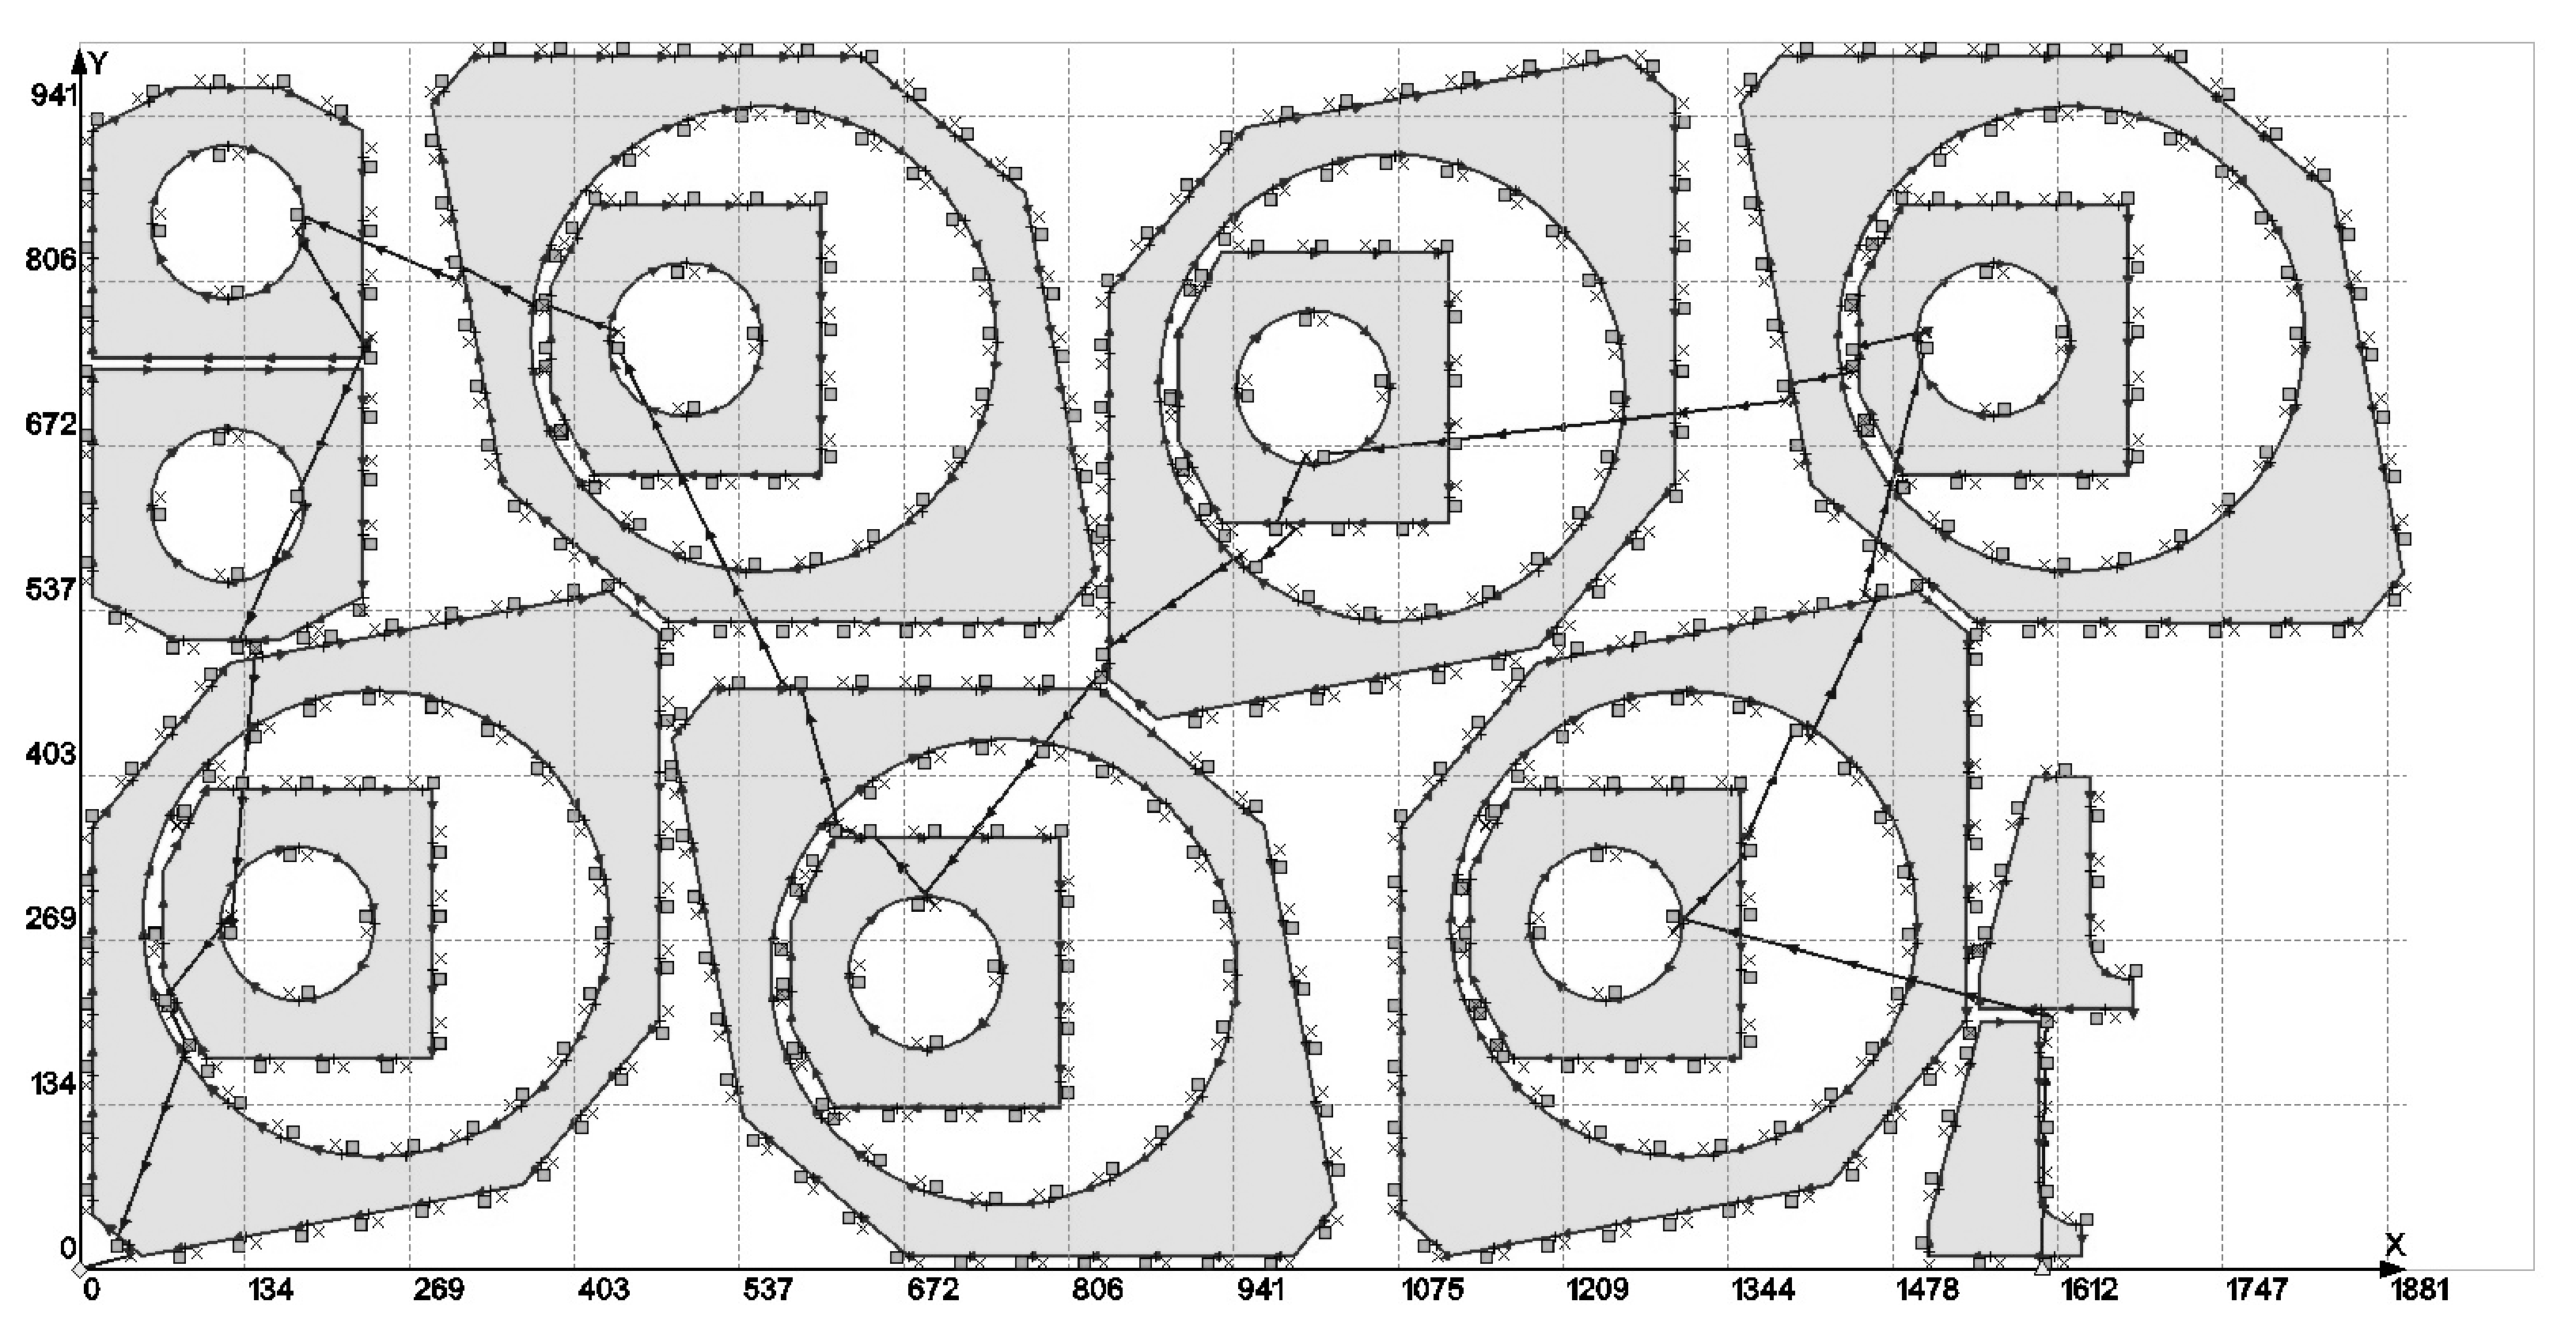
\includegraphics[width=0.9\textwidth]{image.eps}
  \caption{Маршрут и трасса обхода множеств}
  \label{fig:1}
\end{figure}

Модель мегаполисов применима и при использовании нестандартных техник резки,
в частности, т.н. мульти-контурной резки,
которая предполагает использование только одной точки врезки
для вырезки двух и более контуров внутри одного сегмента резки.
Под сегментом резки подразумевается траектория рабочего хода инструмента
между точкой врезки и соответствующей ей точкой выключения инструмента
\cite{100}.
На рис.~\ref{fig:2}
показан пример расчета оптимальной траектории инструмента
при резке 19 деталей, заданных 24-мя контурами.
Для пар деталей, отмеченных цифрами 1--2, 3--4, 5--6
были сформированы три отдельных мегаполиса,
всего 21 мегаполис.
Расчет оптимальной точки старта в данном примере не производился.

\begin{figure}[]
  \centering
  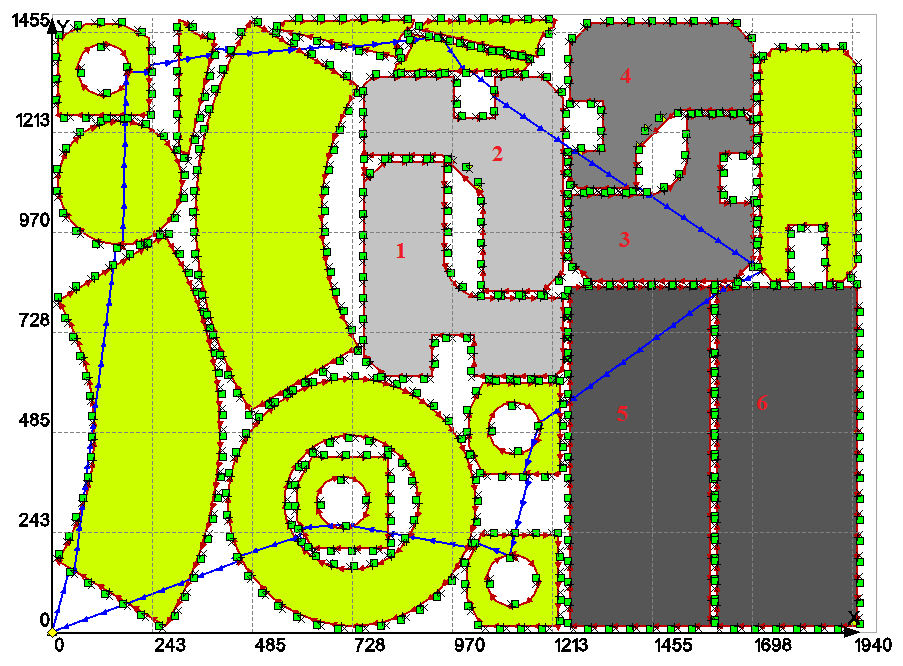
\includegraphics[width=0.9\textwidth]{cut19.png}
  \caption{Оптимальная траектория резки при использовании мульти-контурной техники резки}
  \label{fig:2}
\end{figure}

Следует отметить,
что описанная в статье математическая модель позволяет получать
на обычном персональном компьютере точные варианты решения
для задач маршрутизации инструмента машин листовой резки с ЧПУ
для раскройных карт,
содержащих 30 и более деталей.

\printbibliography[title=Литература]

\begin{aboutAuthors}

\textbf{Петунин Александр Александрович}~---~
д-р техн. наук., доцент;
профессор кафедры информационных технологий и автоматизации проектирования УрФУ.
Число научных публикаций~---~147.
a.a.petunin@urfu.ru,
https://urfu.ru;
Уральский Федеральный университет,
620002, Екатеринбург, Мира, 19.
\smallskip

\textbf{Ченцов Александр Георгиевич}~---~д-р физ.-мат. наук., профессор, член-корреспондент РАН;
главный научный сотрудник, chentsov@imm.uran.ru; Институт математики и механики им Н.Н.Красовского УрО РАН;
Число научных публикаций~---~592.
620990, г.Екатеринбург,
ул. Софьи Ковалевской 16.
Главный научный сотрудник, профессор, Уральский Федеральный университет,
620002, Екатеринбург, Мира, 19.

\smallskip

\textbf{Ченцов Павел Александрович}~---~канд. физ.-мат. наук., старший научный сотрудник, chentsov.p@mail.ru; Институт математики и механики им Н.Н.Красовского УрО РАН.
Число научных публикаций~---~78.
620990, г.Екатеринбург,
ул. Софьи Ковалевской 16.
Старший научный сотрудник,
Уральский Федеральный университет,
620002, Екатеринбург, Мира, 19.
\smallskip

\textbf{Поддержка исследований.}
Работа выполнена при финансовой поддержке РФФИ (грант 20-08-00873).

\end{aboutAuthors}

\end{document}
